\documentclass[tikz]{standalone}
\usepackage{pgfplots}
\pgfplotsset{compat=1.15}
\usepackage{mathrsfs}
\usetikzlibrary{arrows,calc}
\usepackage{tkz-euclide}
\pagestyle{empty}
\usepackage{fp}

\definecolor{AngleClr}{rgb}{0,0.39215686274509803,0}
\definecolor{ShapeClr}{rgb}{0.6,0.2,0}

\begin{document}

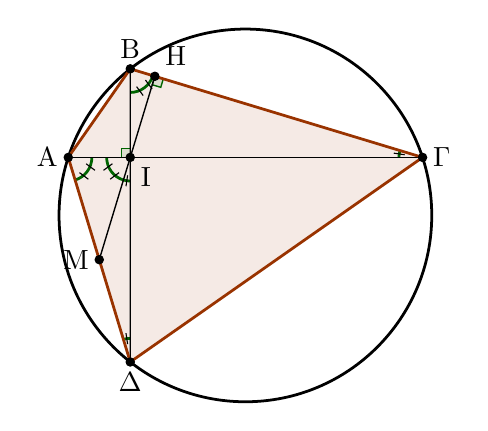
\begin{tikzpicture}[scale=.75]
\tkzSetUpLine[line width=1pt,color=black]
\tkzSetUpPoint[fill=black]

\tkzDefPoints{0/0/A,6/0/C,1.05/1.5/B}

\tkzDefCircle[circum](A,B,C)
\tkzGetPoint{O}
\tkzDrawCircle[line width=1.0pt, color=black](O,A)


% Find the fourth point of the quadrilateral.
\tkzDefLine[orthogonal=through B](C,A) \tkzGetPoint{X_1}
\tkzInterLC(B,X_1)(O,A) \tkzGetSecondPoint{D}

% Find the intersection of the diagonals.
\tkzInterLL(B,D)(A,C) \tkzGetPoint{I}

\tkzFillPolygon[fill=ShapeClr,fill opacity=0.1,inner sep=1cm](A,B,C,D)

\tkzMarkRightAngle[line width=0.5pt, size=.15,color=AngleClr,fill=AngleClr,fill opacity=0.1](B,I,A)

\tkzDefMidPoint(A,D) \tkzGetPoint{M}


\tkzInterLL(M,I)(B,C) \tkzGetPoint{H}

\tkzMarkRightAngle[line width=0.5pt, size=.15,color=AngleClr,fill=AngleClr,fill opacity=0.1](I,H,C)

% Mark angles.
\tkzMarkAngles[mark=|,mksize=2,line width=1pt,size=.4,color=AngleClr](B,D,A B,C,A M,I,D)
\tkzMarkAngles[mark=||,mksize=2,line width=1pt,size=.4,color=AngleClr](D,A,C D,B,C A,I,M)

\tkzDrawSegments[line width=0.5pt,color=black](A,C B,D H,M)


\tkzDrawPolygon[color=ShapeClr](A,B,C,D)
\tkzDrawPoints[size=3](A,B,C,D,I,M,H)
\tkzLabelPoint[left](A){$\rm A$}
\tkzLabelPoint[above](B){$\rm B$}
\tkzLabelPoint[right](C){$\rm \Gamma$}
\tkzLabelPoint[below](D){$\rm \Delta$}
\tkzLabelPoint[below right](I){$\rm I$}
\tkzLabelPoint[above right](H){$\rm H$}
\tkzLabelPoint[left](M){$\rm M$}

\end{tikzpicture}

\end{document}
